\documentclass[11pt]{article}

\newcommand{\numpy}{{\tt numpy}}

\topmargin -.5in
\textheight 9in
\oddsidemargin -.25in
\evensidemargin -.25in
\textwidth 7in
\usepackage{amsmath}
\usepackage{listings}
\usepackage{fancyvrb}
\usepackage{indentfirst}
\usepackage{hyperref}
\usepackage{graphicx}
\graphicspath{ {./} }
\usepackage{multicol}

\begin{document}

\author{Kelompok B09}
\title{Tugas Kelompok Analisis Numerik : Stewart Problem}
\date{Maret 2019}
\maketitle
\medskip

\begin{multicols}{2}
\section{Introduction}
\label{sec:Intro}
\textit{Stewart Platform} adalah sebuah permukaan yang ditopang oleh enam buah kaki dengan panjang yang dapat berubah-ubah dan dihubungkan dengan sendi prismatik. \textit{Stewart Platform} ini biasanya digunakan untuk menciptakan ruang tiga dimensi yang diinginkan oleh suatu objek dengan meletakkan muatan di berbagai titik di berbagai kemiringan. Salah satu contoh pemanfaatan \textit{Stewart Platform} adalah alat simulasi penerbangan (FlightGlobal/Archive, 2019).

\medskip

\textit{Stewart Platform} ini dimungkinkan untuk dianalisis secara sederhana dalam bentuk dua dimensi. \textit{Stewart Platform} digambarkan sebagai sebuah bidang manipulator berbentuk segitiga yang diatur posisinya oleh tiga buah penopang pada bidang \textit{Cartesian}. Bidang manipulator tersebut memiliki sisi $L1$, $L2$ dan $L3$ dengan $\gamma$ adalah sudut yang menghadap ke $L1$; sedangkan panjang tiap penopang dilambangkan dengan $P1$, $P2$ dan $P3$.

\medskip

Dengan bantuan beberapa variabel lain yang akan disebutkan pada bagian \hyperref[sec:Content]{\textbf{Content}}, dalam proyek ini kami ingin menyelesaikan beberapa permasalahan yang disebutkan, antara lain :
\begin{enumerate}
    \item Membuat kode \textit{Octave/Matlab}  dengan parameter bebas $\theta$ dan konstanta lainnya dimana dihipotesiskan $f(\theta) = 0$ saat $\theta = \pi/4$ atau $\theta = -\pi/4$.
    \item Membuat kode Octave/Matlab  untuk plotting $f(\theta)$ di interval [$-\pi, \pi$].
    \item Menghasilkan kembali sebuah pose yang diberikan dengan fungsi \textit{plot} yang ada di Octave/Matlab.
    \item Mencari kemungkinan bentuk pose dari parameter yang telah ditentukan.
    \item Mencari nilai parameter tertentu dari jumlah pose yang telah ditentukan.
\end{enumerate}


\section{Why?}
\label{sec:Why}
Selain untuk mengerjakan tugas dari mata kuliah Analisis Numerik yang kami ambil, kami juga tertarik dengan bagaimana harmonisasi antar penopang yang dapat menciptakan suatu kemiringan pada bidang manipulator. Kami juga tertarik untuk menyelesaikan permasalahan kinetika langsung \textit{Stewart Platform} untuk model dua dimensi.

\section{Content}
\label{sec:Content}
\subsection{Part 1}
Pada bagian ini, kami mengimplementasikan fungsi yang diminta untuk dibuat menjadi sebuah kode. Fungsi ini memiliki parameter bebas $\theta$ sebagai input dan parameter terikat berupa output dari $f(\theta)$. Selain itu, terdapat panjang penopang ($p1, p2, p3$), sisi platform ($L1, L2, L3$) dan sudut \textit{platform} menghadap $L1$ ($\gamma$) yang menjadi konstanta di persamaan ini. Kode yang kami gunakan dapat dilihat pada lampiran yang kami kumpulkan bersama dengan laporan ini (fungsi 1).

\medskip

Setelah itu, untuk menguji kode yang kami buat, kami memasukkan nilai $\theta = \frac{\pi}{4}$ dan $\theta = -\frac{\pi}{4}$ pada fungsi tersebut dengan harapan akan menghasilkan nol. Ternyata kami mendapatkan nilai $f(\theta) = -4.547473508864641e-13$ untuk kedua nilai $\theta$ yang dimasukkan ke dalam fungsi tersebut. Terlihat bahwa nilai tersebut mendekati nol yang berarti fungsi yang kami buat cukup akurat.

\subsection{Part 2}
Untuk membuat plotting fungsi $f(\theta)$ pada $\theta = [-\pi, \pi]$, kami menggunakan kode fplot(@f, [-pi,pi])  yang menghasilkan plot sebagai berikut :

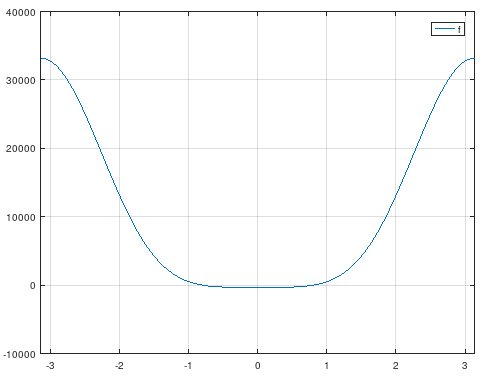
\includegraphics[width=8cm]{plot1.png}

\medskip

Dari gambar diatas, terlihat bahwa terdapat akar (output mendekati nilai nol) pada nilai $\theta = \pm\frac{\pi}{4}$.

\subsection{Part 3}

Disini, kami diminta untuk membuat plot \textit{Stewart Platform} di bidang \textit{Cartesian} (2D) yang sama dengan contoh yang telah diberikan pada soal sebelumnya. Untuk itu, kami membuat kode yang mengimplementasikan fungsi yang dapat menampilkan plot tersebut (fungsi 2). Fungsi yang menerima parameter ber-format $(x1, x2, x3, y1, y2, y3)$ kami masukkan nilai $(1, 2, 2, 2, 1, 3)$ untuk gambar plot pertama dan nilai $(2, 3, 1, 1, 2, 2)$ untuk gambar plot kedua.


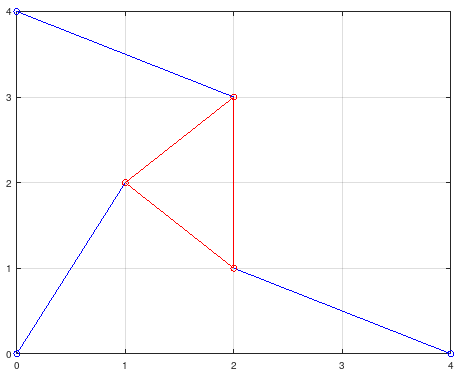
\includegraphics[width=8cm]{plot2.png}

\centerline{Gambar plot pertama}

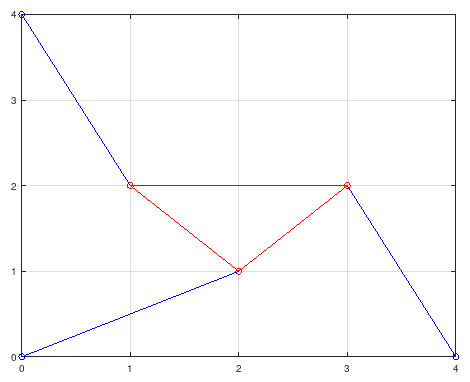
\includegraphics[width=8cm]{plot3.png}

\centerline{Gambar plot kedua} % ini aja lebih pendek sih wkwk ; nice

\subsection{Part 4}

Bagian keempat dari laporan ini menyajikan pemodelan 2 dimensi dari \textit{Stewart Platform} dengan parameter konstan yang diganti dari kode perhitungan sebelumnya dan kami mencoba mencari 4 pose yang berbeda dari \textit{Stewart Platform} tersebut. Sebelum mencari pose - pose tersebut, kami mencoba mencari plot $f(\theta)$ di $\theta = [-pi, pi]$ terlebih dahulu dengan menggunakan (fungsi 3).

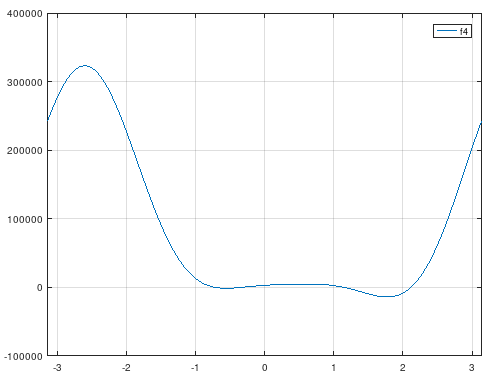
\includegraphics[width=8cm]{plot4.png}
 
 \centerline{plotting $f(\theta)$}
\medskip
%TODO BIKIN JADI ITEM%
Terlihat bahwa grafik fungsi tersebut memiliki empat akar. Keempat akar tersebut akan kami cari nilainya dengan menggunakan \textit{Bisection Method} (fungsi 4). Untuk mendapatkan akar, batas yang kami gunakan berturut - turut adalah $[-1, -0.5]$; $[-0.5, 0]$; $[1, 1.5]$; dan $[2, 2.5]$. Hasil dari pengakaran tersebut adalah :
\begin{itemize}
    \item akar pertama : $x_1=-0.72085$
    \item akar kedua : $x_2=-0.33101$
    \item akar ketiga : $x_3=1.1437$
    \item akar keempat : $x_4=2.1159$
\end{itemize}

Kedua Selanjutnya kami mencari plot dari tiap $\theta$ tersebut menggunakan (fungsi 6) di kode kami.

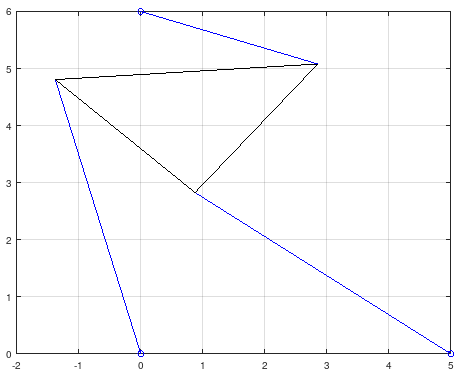
\includegraphics[width=8cm]{plot5.png}

\centerline{$\theta = -0.72085$ dan $(x,y) = (-1.3784, 4.8063)$}

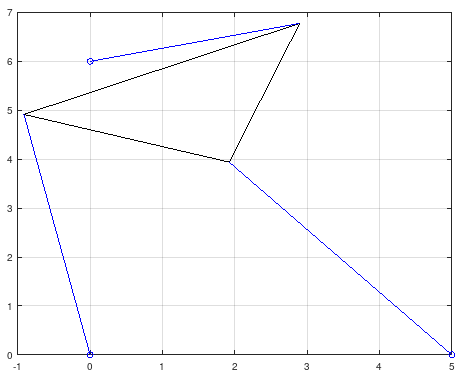
\includegraphics[width=8cm]{plot6.png}

\centerline{$\theta = -0.33101$ dan $(x,y) = (-0.91471, 4.9156)$}

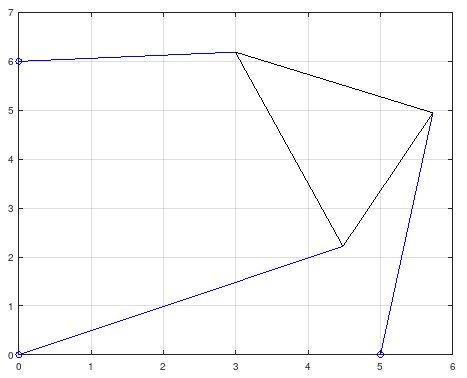
\includegraphics[width=8cm]{plot7.png}

\centerline{$\theta = 1.1437$ dan $(x,y) = (4.4818, 2.2167)$}

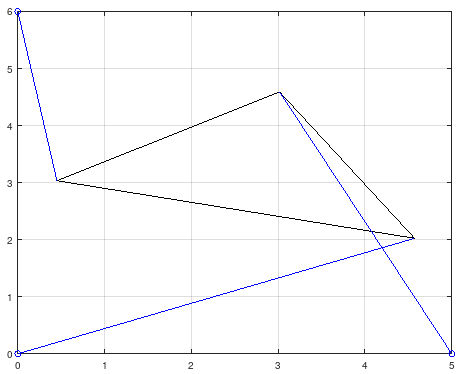
\includegraphics[width=8cm]{plot8.png}

\centerline{$\theta = 2.1159$ dan $(x,y) = (4.5718, 2.0244)$}

\medskip

Perlu diketahui bahwa kode plotting pose \textit{Stewart Platform} yang kami buat di bagian 4 ini akan digunakan hingga bagian 6 dengan beberapa modifikasi kecil.

\subsection{Part 5}
%TODO BAGUSIN KALIMATNYA%
Sama seperti di bagian 4, di bagian ini kami mencari grafik dari fungsi yang diimplementasikan ke kode kami. Ide kami adalah mencari terlebih dahulu plot dari fungsinya dan melihat kemungkinan nilai dari akar-akarnya.

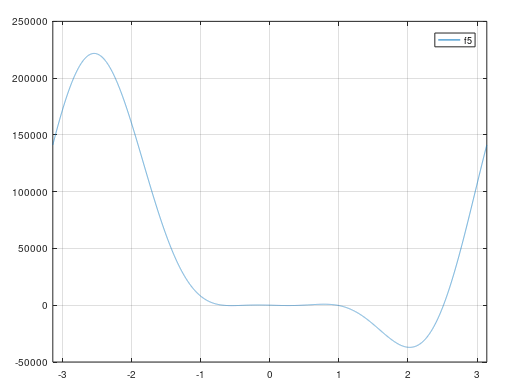
\includegraphics[width=8cm]{Plot9.PNG}
\centerline{Plotting $f(\theta)$}

\medskip

Lalu dengan metode \textit{bisection} akan dicari nilai akar-akar dari fungsi tersebut yang selanjutnya akan kami gunakan sebagai parameter $\theta$ dari fungsi \textit{Stewart Plot} yang telah kami buat sebelumnya.

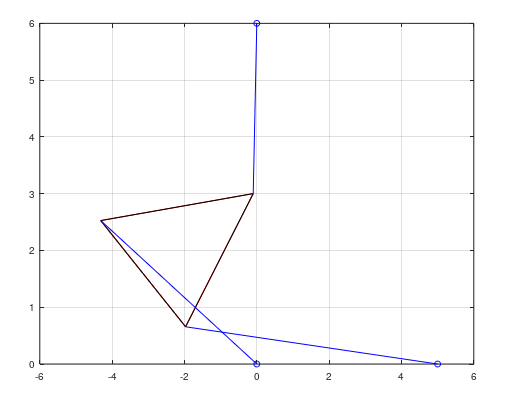
\includegraphics[width=8cm]{Plot10.PNG}

Batas $[-0.8,-0.6]$, $\theta=-0.67316$, $(x,y)=(-4.3148,2.5264)$

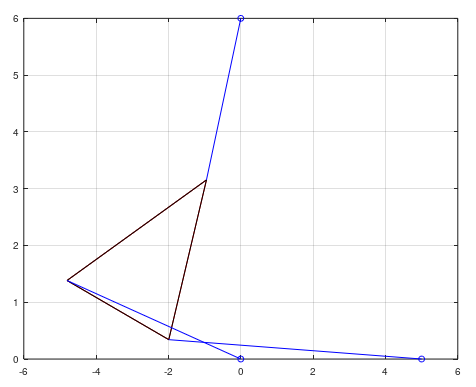
\includegraphics[width=8cm]{Plot11.PNG}

Batas $[-0.6,-0.2]$, $\theta=-0.35474$, $(x,y)=(-4.8049,1.3831)$

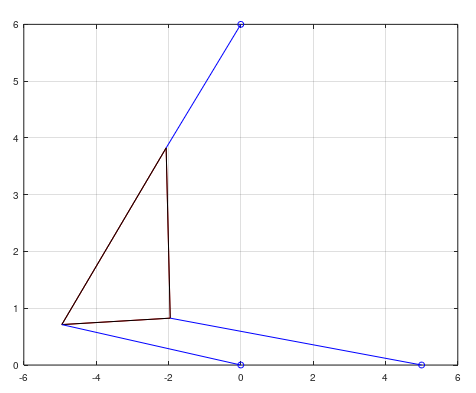
\includegraphics[width=8cm]{Plot12.PNG}

Batas $[-0.2, 0.2]$, $\theta=0.037767$, $(x,y)=(-4.9490,0.71215)$

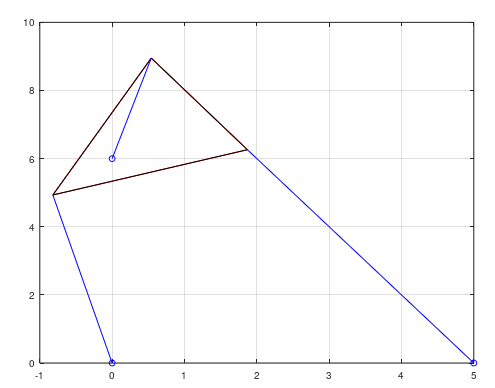
\includegraphics[width=8cm]{Plot13.PNG}

Batas $[0.2, 0.6]$, $\theta=0.45888$, $(x,y)=(-0.81980,4.9323)$

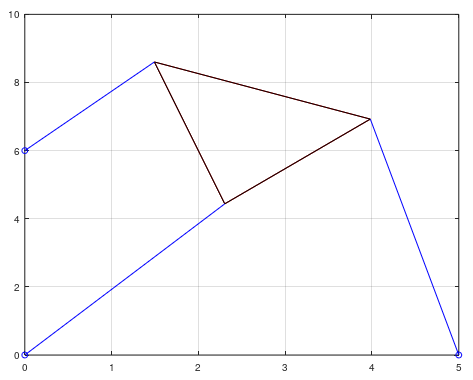
\includegraphics[width=8cm]{Plot14.PNG}

Batas $[0.6, 1.2]$, $\theta=0.97767$, $(x,y)=2.3036, 4.4378$

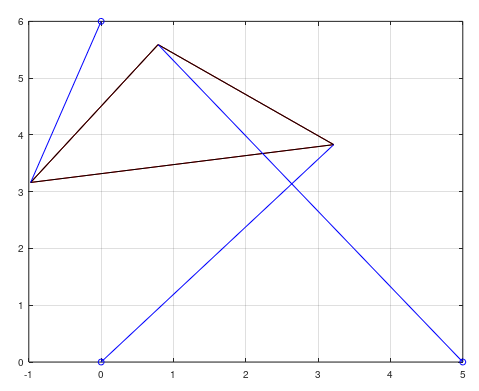
\includegraphics[width=8cm]{Plot15.PNG}

Batas $[1.2, 2.6]$, $\theta=2.5139$, 
$(x,y)=(3.2157,3.8287)$

\subsection{Part 6}
%TODO BAGUSIN KALIMATNYA%
Pada nomor 6, kami membuat algoritma untuk mencari nilai yang dapat merepresentasikan $\theta$ sehingga $f(\theta) = 0$ dan mampu menghasilkan tepat 2 buah pose \textit{Stewart Platform} dengan memanfaatkan \textit{Intermediate Value Theorem}.

\medskip

Kami melakukan mengimplementasikan fungsi bersifat \textit{brute force} (fungsi 10) terhadap nilai $p2$ untuk mencari berapa kali $f(\theta)$ bernilai $0$ dengan menghitung berapa kali output dari algoritma kami berubah tanda (positif <-> negatif). Ketika fungsi tersebut berganti tanda sebanyak dua kali, maka fungsi $f(\theta)$ sudah bernilai $0$ sebanyak dua kali. Dengan demikian, dua buah akar akan ditemukan dan dapat dibuat tepat 2 buah pose.

\medskip

Dari perhitungan fungsi tersebut, kami menemukan bahwa nilai $p2 = 9.2$ akan menghasilkan tepat 2 buah pose. Selanjutnya kami memasukkan nilai $p2 = 9.2$ sebagai $p2$ dari (fungsi 11) untuk membuat plotnya terhadap $[-\pi, \pi]$.

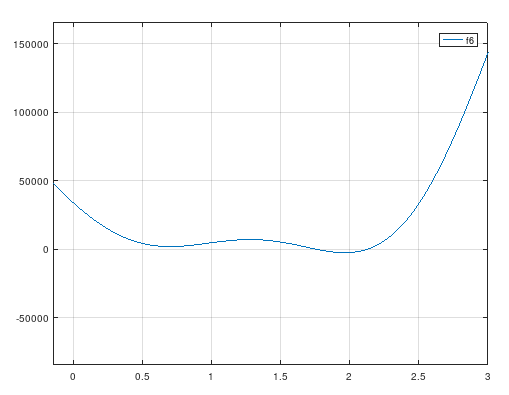
\includegraphics[width=8cm]{cuk.png}

\subsection{Part 7}
%TODO BELUM DICEK%
Pengerjaan nomor 7 merupakan kelanjutan dari nomor 6, dimana kami mencoba mengimplementasikan metode \textit{brute force} terhadap $p2$ untuk mendapatkan interval-interval yang memiliki jumlah akar yang genap. menggunakan (fungsi 13), kami mendapatkan hasil sebagai berikut : 

%gah
%gah
%gak perlu plotting ya yg nomor 6?
\begin{enumerate}
    \item interval $0 - 3.7150000000$ : 0 akar
    \item interval $3.7150000000 - 4.865000000$ : 2 akar
    \item interval $4.8650000000 - 6.970000000$ : 4 akar
    \item interval $6.9700000000 - 7.025000000$ : 6 akar
    \item interval $7.0250000000 - 7.850000000$ : 4 akar
    \item interval $7.8500000000 - 9.265000000$ : 2 akar
    \item interval $9.2650000000 - \infty$ : 0 akar
\end{enumerate}



\section{Conclusion}
\label{sec:Conclusion}

Dari aktivitas yang kami lakukan di atas, kami merasa senang karena telah berhasil memodelkan \textit{Stewart Platform} dalam model dua dimensi. Kami menemukan banyak kesulitan sepanjang melakukan aktivitas ini, contohnya adalah dalam hal plotting dan mencari nilai-nilai $\theta$ dari suatu fungsi. Kami menarik kesimpulan bahwa banyaknya pose dari suatu \textit{Stewart Platform} bergantung dari banyaknya akar-akar dari fungsi $f(\theta)$ tersebut.

\end{multicols}

\section{Reference}
\label{sec:Reference}
\begin{enumerate}
    \item Bouck, Lucas, et al. (2016). \textit{Project 1}. Retrieved from http://mason.gmu.edu/~lbouck/project1.html
    \item Sauer, Timothy (2012). \textit{Numerical Analysis}. Boston, MA: Pearson Education
\end{enumerate}

\end{document}
